\section{Experiments}

\subsection{Training and Testing Dataset}
\label{sec:traintest}
\begin{singlespace}
\begin{figure}[H]
	\centering
	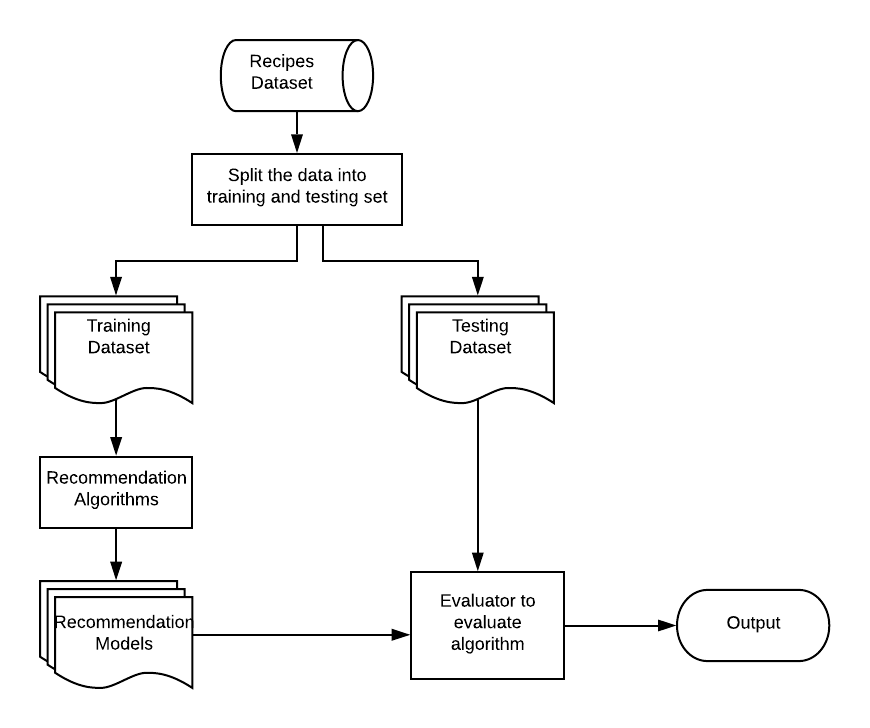
\includegraphics[width=0.75\linewidth]{overview_train_test_evaluation}
	\caption{Train Test Evaluation }
	\label{fig:overview_train_test_evaluation}
\end{figure}  
\end{singlespace}
The overview of training and testing dataset is given in \autoref{fig:overview_train_test_evaluation}. The full dataset was randomly split into
two parts - training dataset and testing dataset. The 80\% of the data was split into training dataset while 20\% comprises of testing set.  
The training data set was fed to the algorithm to build a model and then built model was evaluated on the test dataset to calculate recall, precesion and accuracy for experiments. Recall, precision and accuracy evaluation matrics are discussed in the section \nameref{sec:eval_metrics}. \\
Data statistics used for the experiments include:\\
\begin{itemize}
\item Total number of Recipes = 43,922
\item Total number of users = 10,000
\item Total number of user-recipe interactions = 162,019
\end{itemize}



\subsection{Experiment 1}
\label{sec:cb_ingred_exp}
The purpose of this experiment was to evaluate user recommendations using content-based algorithm on ingredients described in the section \nameref{sec:cb_ingredients}. For this experiment, \lq{}Ingredients\rq{} attribute is used. The training and testing datasets are split as explained in the section \nameref{sec:traintest}. The experiment was performed for an output set of 5, 10 and 20 recommendations. 

\subsection{Experiment 2}
\label{sec:cb_ingred_cook_method_exp}
The purpose of this experiment was to evaluate the user recommendations using content-based algorithm on ingredients and cook method described in the \nameref{sec:cb_ingredients_cook_method}. For this experiment, \lq{}Ingredients\rq{} and \lq{}Cook Method\rq{} attributes are used. The training and testing datasets are split as explained in the section \nameref{sec:traintest}. The experiment was performed for an output set of 5, 10 and 20 recommendations.

\subsection{Experiment 3}
\label{sec:cb_ingred_cook_method_diet_label_exp}
The purpose of this experiment was to evaluate the user recommendations using content-based algorithm on ingredients, cook method  and diet labels described in the \nameref{sec:cb_ingredients_cook_method_diet_labels}. For this experiment, \lq{}Ingredients\rq{}, \lq{}Cook Method\rq{} and \lq{}Diet Label\rq{} attributes are used. The training and testing datasets are split as explained in the section \nameref{sec:traintest}. The experiment was performed for an output set of 5, 10 and 20 recommendations.

\subsection{Experiment 4}
\label{sec:cf_exp}
The purpose of this experiment was to evaluate the user recommendations using collaborative filtering - SVD algorithm. Ratings given to recipes were extracted from the dataset and unrated combinations of user and recipes were predicted as mentioned in section \nameref{sec:cf}. \nameref{sec:cf_exp} determined the recall, precision and accuracy of the results on randomly generated testing dataset. The experiment was performed for an output set of 5, 10 and 20 recommendations.

\subsection{Experiment 5}
\label{sec:hybrid_exp}
The purpose of this experiment was to evaluate the user recommendations using combination of content-based model that consists of ingredients, cook method, diet labels and collaborative filtering - SVD algorithm. Recommendations from content-based and collaborative filtering are combined by applying weightage as described in \nameref{sec:hybrid_impl}
\nameref{sec:cf_exp} determined the recall, precision and accuracy of the results on randomly generated testing dataset. The experiment was performed for an output set of 5, 10 and 20 recommendations.